\documentclass[a4paper,UTF8]{article}
\usepackage{ctex}
\usepackage[margin=1.25in]{geometry}
\usepackage{color}
\usepackage{graphicx}
\usepackage{amssymb}
\usepackage{amsmath}
\usepackage{amsthm}
%\usepackage[thmmarks, amsmath, thref]{ntheorem}
\theoremstyle{definition}
\newtheorem*{solution}{Solution}
\newtheorem*{prove}{Proof}
\usepackage{multirow}
\usepackage{url}
\usepackage[colorlinks,urlcolor=blue]{hyperref}
\usepackage{enumerate}
\renewcommand\refname{参考文献}


%--

%--
\begin{document}
\title{\textbf{《计算机图形学》 6月报告}}
\author{161220062 李奡程 \href{mailto:xxx@xxx.com}{161220062@smail.nju.edu.cn}}
\maketitle

\section{综述}
\paragraph{完成的内容} 完成了全部大作业内容,包括线元、多边形、椭圆和两种曲线的生成,上述图元的平移、旋转、缩放和线段的裁剪,并在前后端分离的基础上分别开发了命令行界面和图形界面。
\section{算法介绍}
\subsection{线画图元介绍}
\paragraph{Digital Differential Analyzer} 数字差分分析,每次根据斜率在一个坐标轴上以单位间隔对线段取样($\Delta x=1$或$\Delta y=1$),据其计算另一个坐标轴上最靠近线段路径对应的整数值,以此作为最后生成的线元的整点\cite{graphTextBook}。记斜率为$m$,若$|m|>1$,则对于间隔$\Delta x=1$,顺序y值可计算为:
\begin{equation}
y_{k+1}=y_k+m
\end{equation}
对$|m|\leq 1$类似有
\begin{equation}
x_{k+1}=x_k+\frac{1}{m}
\end{equation}
\par 然而,实际实现时,可能存在直线垂直于x轴或y轴的情况,我采用的办法是特殊处理,保证斜率取值合法再进行DDA,否则只用在某一条平行线上赋值,这样的话存在高效存取方法实现。
\paragraph{Bresenham算法} 详细算法课本上有,所以在此用我的语言归纳总结一下,其针对DDA中可能出现的累积误差的问题,选择使用决策函数来在每一点决定下一个点时的选择,并通过动态更新决策函数有力的消除了累计误差的问题,而且其全部使用整数计算,开销比全部使用浮点数的DDA大大减少。
\par 具体的,对于第一象限的直线,斜率小于1时,在点$(x_k,y_k)$处,$p_k$的更新公式为
\begin{equation}
p_{k+1}=\left\{
\begin{array}{ll}
p_k+2\Delta y-2\Delta x & p_k>0 \\
p_k+2\Delta_y & p_k<0 \\
\end{array}
\right.
\end{equation}
且初始化其为
\begin{equation}
p_0=2\Delta y-\Delta x
\end{equation}
而对于其他象限以及其他斜率的直线,可对应变换$x$,$y$,$p_k$的相应项完成。由于象限间的对称性,在我实现中通过规定$y$的相对关系将需要处理的情况减为4种,再通过对称性仅处理两种情况即可。
\paragraph{测试}
\begin{figure}
	\centering
	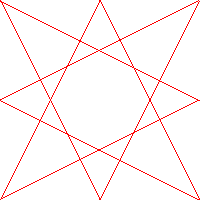
\includegraphics[height=6cm]{1.png}
	\caption{Bresenham 测试图样}
	\label{testLine}
\end{figure}
由于Bresenham需要处理8种情况,所以应该使测试用例覆盖8个朝向的边保证正确地覆盖所有可能。我使用了图\ref{testLine}中的八条线来检测,其结果清晰可见,并且能很快的显示出错误的可能原因,加速了我的debug过程。上图也用于检测DDA的实现的正确性。
\subsection{多边形}
\paragraph{绘制} 由于多边形可以视为由若干条直线构成,所以在此我复用线的相关算法,将多边形的各个边画分别画好即完成绘制。注意到多边形接受输入时可能有重点,所以处理时特判即可。
\subsection{椭圆}
\paragraph{中点圆生成算法} 即为Bresenham算法,借鉴Bresenham累积误差的思想,以及利用椭圆的对称性,通过第一象限中分割为斜率的绝对值小于1的两部分,并在各部分通过一边每次加一、另一边用判断函数决定位置来减少累积误差。以下讨论第一象限的处理情况,设曲线解析式为$\frac{x^2}{a^2}+\frac{y^2}{b^2}=1$,且$a>b$,则使用齐次坐标时该曲线表示为
\begin{equation}
\mathbf{C}=\left(
\begin{array}{ccc}
b^2 & 0 & 0 \\
0 & a^2 & 0 \\
0 & 0 & -a^2b^2 \\
\end{array}
\right)
\end{equation}
其中$\mathbf{C}$满足$\mathbf{x}^T\mathbf{C}\mathbf{x}=0$。由参考书知,曲线C在某一点$\mathbf{x}=(x_0,y_0,1)^T$处的切线即为$\mathbf{Cx}$,使该点斜率为1,可得
\begin{equation}
b^2x_0=a^2y_0
\end{equation}
带回曲线解析式,可得交点坐标为$(\frac{a^2}{\sqrt{a^2+b^2}},\frac{b^2}{\sqrt{a^2+b^2}})$,即在$0\leq x\leq x_0$段上,y的斜率的绝对值恒小于1,故每次增加x判断y;在$x_0\leq x\leq a$段上,y的斜率的绝对值恒大于1,故每次减少y判断x。
\par 而对于第一部分,我们使用椭圆决策函数判断,其表达式为
\begin{equation}
p_{1k}=f_{ellipse}(x_{k+1},y_k-\frac{1}{2})=b^2(x_k+1)^2+a^2(y_k-\frac{1}{2})^2-a^2b^2
\end{equation}
若$p_{1k}<0$,则中点位于椭圆内,$y_{k+1}=y_{k}$不变;反之则$y_{k+1}=y_k-1$。联立,可得判断条件为
\begin{equation}
\left\{
\begin{array}{ll}
p_{1k+1}=p_{1k}+2b^2x_k+3b^2 & p_{1k}<0 \\
p_{1k+1}=p_{1k}+2b^2x_k-2a^2y_k+2a^2+3b^2 & p_{1k}\geq 0 \\
\end{array}
\right.
\end{equation}
\par 对于区域2,此时决策函数变为
\begin{equation}
p_{2k}=f_{ellipse}(x_{k}+\frac{1}{2},y_k-1)=b^2(x_k+\frac{1}{2})^2+a^2(y_k-1)^2-a^2b^2
\end{equation}
同时相应修改判断条件。得到第一象限表示后,将其对称投影到剩下三个象限,即得到最后的椭圆。
\subsection{曲线}
\paragraph{Bezier曲线}
\paragraph{B样条曲线}
\subsection{图元的平移}
\subsection{图元的旋转}
\subsection{图元的缩放}
\subsection{线段裁剪}
\section{系统介绍}
\paragraph{总体架构} 其分为命令行界面和图形界面两部分,分别位于两个文件夹下,命令行界面主要由四部分构成:
\subparagraph{main} 接收用户输入,显示相关信息;
\subparagraph{parser} 作为命令行前端,分析用户输入,进行基础的词法语法分析,拒绝非法输入,并将合法输入传到画图后端进行处理;
\subparagraph{panel} 其为画板,作为系统中间层,调用各种图元以完成各种图形操作,同时按照前端要求显示与保存图片。使用其作为中间层能够有效的屏蔽后端实现细节,并且直接作为GUI的中间层加以使用,而不用特别修改相应算法。
\subparagraph{各种图元} 在一个月的学习后,以及受到sklearn中类设计的启发,我意识到实际上可以将后端的功能进一步分离,只要设计好每种图元自身的数据结构,并使其支持draw,scale,rotate等操作(线段还要再支持clip操作),就可以直接通过panel保存图元字典来直接调用,实现更好的数据封装。目前相关实现在commandLine/Line.py,Polygon.py, Ellipse.py 和 Curve.py中,其为CLI和GUI共同的后端核心代码。
\par 而图形界面部分使用PyQt完成,选择PyQt的原因是其提供了一个强大易写的前端接口,同时能兼顾之前书写的代码。其主要分为三部分:
\subparagraph{main} GUI的主窗口,包括各种交互界面,部件间的连接关系等;
\subparagraph{displayLabel} 重写后的QLabel类,其作为与用户交互的最前端,接受分析Mouse Press Event和Mouse Release Event获取用户输入,并传回main窗口进行相应操作,最后再将处理好的图片显示再QLabel上,完成整个交互过程;
\subparagraph{各种图元} 这里直接复用CLI中的相关部分,因为我们只需要调用它的接口,而不需对相关逻辑做出任何改动。
\paragraph{运行}
命令行界面部分在commandLine文件夹下python main.py或者./main.py即可运行。可使用./main.py input.txt 或者 ./main.py $<$ input.txt 读取测试文件输入运行,查看效果。GUI部分在gui文件夹下,同样使用python main.py或者./main.py运行。其不接受读入文件,而是直接通过图形界面进行交互。
\par 另外执行./main.py后进入交互界面,可以通过show指令展示当前的画布,并使panel同步图元信息到画布上。具体的运行细节详见系统说明书。
\section{总结}
\paragraph{} 终于完成了整个画图项目,感觉还是收获颇多,
\begin{thebibliography}{2019}
\bibitem{graphTextBook} 计算机图形学教程\quad 孙正兴主编\quad 周良,郑洪源,谢强编著
\end{thebibliography}

\end{document}